One of the most important parts of this thesis is the design of the BT algorithm. This chapter aims to present the design we created and provide the reasoning behind it.

\section{Creating a behavior tree structure}
    First, we need to choose the correct approach to designing the BT structure. There are several possible approaches to creating a BT structure. We will discuss a few of these approaches and state the used one. The insight from \cite{BT_creation}, was instrumental for the selection and overview in this section.\\
    The first approach is creating the complete BT structure by hand. Meaning we have to design every node, its position, and its function within the structure. This approach is the easiest but more time-consuming and error-prone than others.\\
    The second approach is creating an initial BT and letting RL algorithms improve the BT's functionality and optimality. There are several options for this particular approach, as multiple possible RL algorithms exist for this task.\\
    The third possible approach is constructing the BT from previously recorded human behavior. This approach also uses RL algorithms to transform the recorded behavior into a BT structure.\\
    The last possible approach lets an RL algorithm construct the BT structure from the ground up.\\
    Each of the presented approaches has its advantages and disadvantages. It is, therefore, vital to select the correct approach based on the possibilities and requirements of the task.\\\\
    \bfc{Chosen approach}\\
        We have chosen the first approach, meaning we will construct the whole tree structure by hand. This was done as it is the easiest approach to this task and requires no additional steps.\\
        Using different approaches to designing and improving the BT structure may be an interesting task for future work.\\
        We will design the BT structure in the GUI application designed alongside our chosen BT library, Groot. The application's interface is shown in figure \ref{fig:groot}.\\\\
        \begin{figure}[ht]
            \centering
            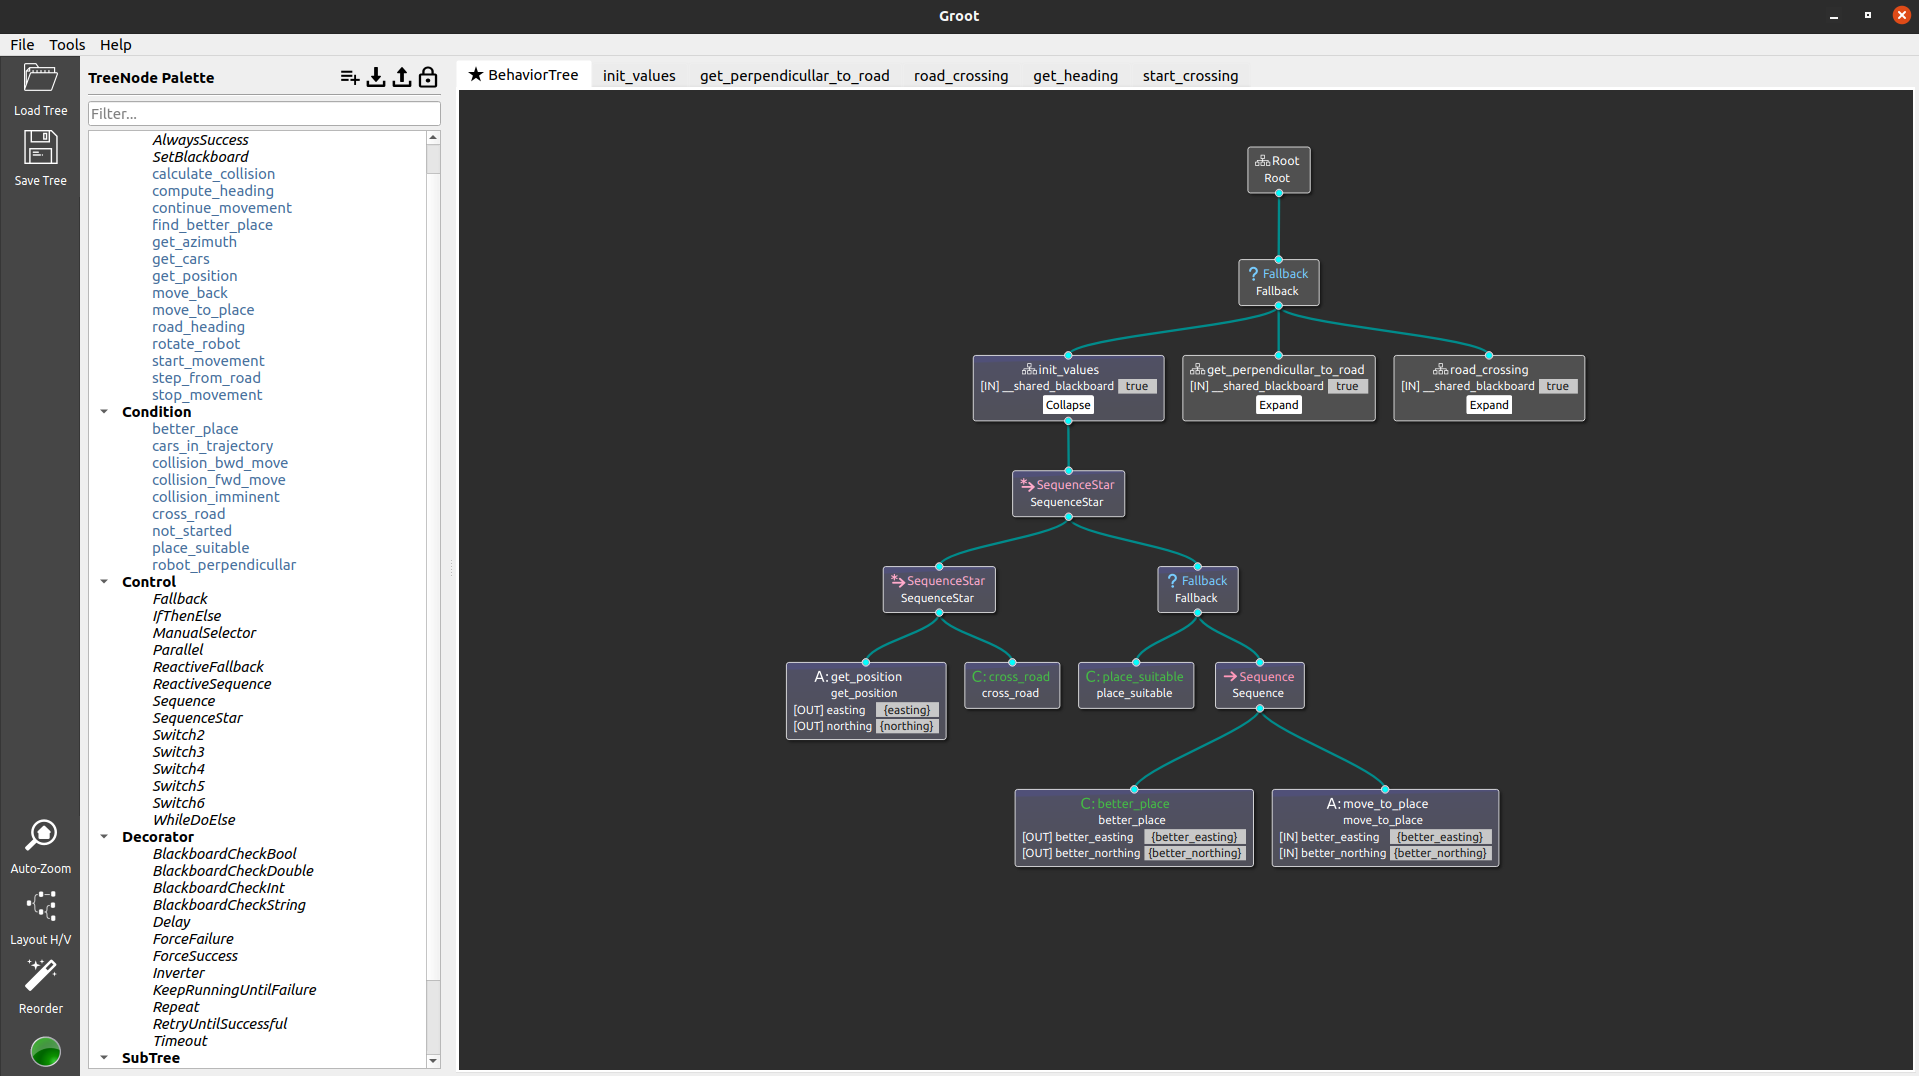
\includegraphics[width=\linewidth]{images/Groot.png}
            \caption{The Groot application interface.}
            \label{fig:groot}
        \end{figure}
    
\section{Structure hierarchy -- Main BT}
    We will divide the whole tree structure into several sub-trees to help with readability, modularity, and maintainability.\\
    The first sub-tree will accomplish the initialization and will be responsible for determining whether the crossing should commence. It is also responsible for navigating the robot to a suitable crossing place. This sub-tree will be called \texttt{Init-BT}.\\
    The second sub-tree is responsible for positioning the robot such that it is perpendicular to the road it is trying to cross. This sub-tree will be called \texttt{Perpendicular-BT}.\\
    The third sub-tree is responsible for the navigation of the robot during the crossing. It will check the position and velocity of incoming traffic and determine the best strategy for the crossing. This sub-tree will be called \texttt{Crossing-BT}.\\
    There are a few more sub-trees in our structure, but as those are not the main ones, we will not present them here. They will be presented when they are mentioned in the main sub-trees structure. Their main task is to help with the modularity and reusability of the behavior they encode.\\
    The main BT is shown in figure \ref{fig:main-BT}.\\
    \begin{figure}[ht]
        \begin{tikzpicture}[sibling distance=30mm, minimum width=1cm, minimum height=0.8cm]
            \node [draw] {$Root$}
                child {node [draw] {$\to$} edge from parent [-{Stealth[length=2.5mm]}]
                child {node [ellipse, draw] {\texttt{StartAlgorithm}}}
                child {node [draw] {$\to^{*}$}
                child {node [draw] {$\to^{*}$}
                child {node [diamond, draw, aspect=2.3, xshift=0-0.5cm, yshift=0-0.5cm] {\texttt{Init}}}
                child {node [diamond, draw, aspect=2.9, yshift=0-0.5cm] {\texttt{Perpendicular}}}}
                child {node [diamond, draw, aspect=2.3] {\texttt{Crossing}}}}};
        \end{tikzpicture}
        \caption{Main BT structure.}
        \label{fig:main-BT}
    \end{figure}
    The main BT starts with a \texttt{Sequence} node. First, we need to check if the algorithm should be even started -- to avoid collision between two nodes trying to control the robot. This we achieve with a condition node \texttt{StartAlgorithm}. This node will check if the algorithm should be started. If it should not, the algorithm will not progress. The second child is a \texttt{SequenceStar} node. This node will tick the sub-trees responsible for the whole algorithm.\\
    However, the first child is again a \texttt{SequenceStar} node. This is done to ensure that each preparation sub-tree will be executed only once, providing they return \texttt{SUCCESS}.\\
    The first preparation sub-tree is the \texttt{Init-BT}, its structure shown in chapter \ref{sec:Init-BT} and its implementation in chapter \ref{sec:Init-BT-impl}.\\
    The second preparation sub-tree is the \texttt{Perpendicular-BT}, its structure shown in chapter \ref{sec:Perpendicular-BT} and its implementation in chapter \ref{sec:Perpendicular-BT-impl}.\\
    The last sub-tree is the \texttt{Crossing-BT}, its structure shown in chapter \ref{sec:Crossing-BT} and its implementation in chapter \ref{sec:Crossing-BT-impl}.

\section{Init BT}
\label{sec:Init-BT}
    As mentioned earlier, this BT is responsible for determining if we should start the crossing and for navigating the robot to the optimal location. This tree will be executed only once for each crossing. The \texttt{Init-BT} structure is shown in figure \ref{fig:Init-BT}.\\
    \begin{figure}[ht]
        \begin{tikzpicture}[sibling distance=28mm, minimum width=1cm, minimum height=0.8cm]
            \node [draw] {$Root$}
                child {node [draw] {$\to$} edge from parent [-{Stealth[length=2.5mm]}]
                child {node [draw, xshift=0-1.6cm] {$\to^{*}$}
                child {node [draw] {\texttt{GetPosition}}}
                child {node [ellipse, draw] {\texttt{CrossRoad}}}}
                child {node [draw, xshift=1.6cm] {?}
                child {node [ellipse, draw, xshift=0.4cm] {\texttt{PlaceSuitable}}}
                child {node [draw, xshift=0.3cm] {?}
                child {node [draw, xshift=0-0.2cm] {$\to$}
                child {node [ellipse, draw, xshift=0-0.2cm] {\texttt{BetterPlace}}}
                child {node [draw, xshift=0.1cm] {\texttt{MoveToPlace}}}}
                child {node [draw, xshift=0-0.4cm] {\texttt{GetBetterPlace}}}
                child {node [ellipse, draw, xshift=0-0.9cm] {$\checkmark$}}}}};
        \end{tikzpicture}
        \caption{The Init-BT structure.}
        \label{fig:Init-BT}
    \end{figure}
    The ticking of nodes in the structure is done in the following way. We start at a \texttt{Sequence} node. With its first child, a \texttt{SequenceStar} control node, we start the \texttt{Init-BT}'s first branch. The first node in this branch is an action node \texttt{GetPosition} followed by a condition node \texttt{CrossRoad}. The idea behind this branch is to determine the proximity of the robot to the road. If the robot is too far away from the road, the algorithm should not progress. This will help combat the possibility of trying to cross the wrong road, should it happen that two roads are close by.\\
    The second branch of this sub-tree starts with a \texttt{Fallback} node. The goal of this branch is to place the robot in an ideal position for crossing. This action should have been done before the mission, and the robot should have been sent to the optimal location by a path-planning node.\\
    However, if such pre-mission planning was not performed, the \texttt{PlaceSuitable} condition node will check if the place is suitable. If not, the \texttt{BetterPlace} condition node will return if a better location has already been found. An action node \texttt{MoveToPlace} will steer the robot to a better location if it has been found. If it has not, the action node \texttt{GetBetterPlace} will try to find a more suitable place.\\
    We will not perform the sub-tree again if a better place cannot be located. Instead, we will move on to the following sub-tree and cross the road in the position the robot is currently situated. This is done to avoid an infinite loop and is achieved with a \texttt{ReturnSuccess} node at the end of the second branch.

\section{Perpendicular BT}
\label{sec:Perpendicular-BT}
    This sub-tree is responsible for positioning the robot in the most optimal way for crossing the road. We have determined that to be the one in which the robot will cross the road the fastest. As such, the robot's heading should be perpendicular to the road it will cross. Figure \ref{fig:Perpendicular-BT} shows the BT structure for achieving so.\\
    \begin{figure}[ht]
        \begin{tikzpicture}[sibling distance=28mm, minimum width=1cm, minimum height=0.8cm]
            \node [draw] {$Root$}
                child {node [draw] {$\to^{*}$} edge from parent [-{Stealth[length=2.5mm]}]
                child {node [draw] {$\to^{*}$}
                child {node [draw] {$\circ(10)$}
                child {node [draw] {\texttt{GetAzimuth}}}}
                child {node [draw, xshift=0-0.7cm] {$\circ(10)$}
                child {node [draw] {$\to$}
                child {node [draw, xshift=0.8cm] {\texttt{GetPosition}}}
                child {node [draw, xshift=0.6cm] {\texttt{RoadHeading}}}
                child {node [draw, xshift=0.7cm] {\texttt{ComputeHeading}}}}}}
                child {node [draw, xshift=3cm] {$\circ(10)$}
                child {node [draw] {$\to$}
                child {node [draw] {\texttt{GetAzimuth}}}
                child {node [draw] {?}
                child {node [ellipse, draw, xshift=0-0.6cm, yshift=0-1.5cm] {\texttt{RobotPerpendicular}}}
                child {node [draw] {$\times$}
                child {node [draw] {?}
                child {node [draw, xshift=0-1.3cm] {\texttt{RotateRobot}}}
                child {node [draw, xshift=0-1.4cm] {\texttt{StepFromRoad}}}}}}}}};
        \end{tikzpicture}
        \caption{The Perpendicular-BT structure.}
        \label{fig:Perpendicular-BT}
    \end{figure}
    The first branch of this tree only needs to be ticked once in each run of the crossing algorithm. Therefore, we have a \texttt{SequenceStar} control node after the \texttt{Root} node.\\
    The primary responsibility of the first branch is to calculate the azimuth that will position the robot perpendicular to the road. As obtaining the robot's azimuth does not need to be repeated once successful, we start the branch with a \texttt{SequenceStar} node. The node has two children, both being a \texttt{Repeat} control node. The action to be repeated behind the first node is the obtaining of the robot's azimuth. The actions behind the second \texttt{Repeat} node are connected in a \texttt{Sequence}. This part of the algorithm calculates the optimal azimuth for the robot. Firstly we need to obtain the robot's position -- \texttt{GetPosition} action node. Next, we need to determine the heading of the road closest to the robot. For this purpose, we have the action node \texttt{RoadHeading}. Finally, we calculate the optimal heading for the robot with the action node \texttt{ComputeHeading}. This concludes the left branch of our Perpendicular-BT.\\
    The right branch starts with a \texttt{Repeat} node, followed by a \texttt{Sequence} node. The idea behind this branch is to utilize the heading value computed in the left branch and orient the robot accordingly. Firstly we need to obtain the robot's azimuth with the \texttt{GetAzimuth} action node. While this might seem redundant, we have just got the azimuth for calculation, it is vital to update the current azimuth as the value of obtained azimuth is only valid in the first run of the second branch. After receiving the current azimuth, we follow with a \texttt{Fallback} node and its first child, a condition node \texttt{RobotPerpendicular}. This node tells us if the robot has achieved the optimal heading we calculated earlier. If not, we continue to the last part of this sub-tree.\\
    The last part shall always return \texttt{FAILURE} and is responsible for the movement of the robot. This is necessary because we check the correct position before the movement. Firstly we try to rotate the robot with an action node \texttt{RotateRobot}. If the rotation was unsuccessful, we try to move the robot away from the road with an action \texttt{StepFromRoad}. The last action is a precaution, as the robot's rotation might have moved the robot onto the road, which is forbidden.\\
    While we could unite the first two \texttt{Repeat} nodes, maybe even all three, we chose not to do so. The reason for not merging the nodes is to allow each part of the algorithm to fail independently. The number of repetitions for each node was set to 10, which we determined to be the optimal value.

\section{Crossing BT}
\label{sec:Crossing-BT}
    This tree is the most important part of the whole algorithm as it facilitates the road crossing. Figure \ref{fig:Crossing-BT} shows the structure of the sub-tree.\\
    This tree starts with a \texttt{Sequence} node with three children. In the structure of this tree, there are two further sub-trees. These sub-trees are shown in figures \ref{fig:StartMovement-BT} and \ref{fig:Finished-BT}, and will be explained separately at the end of this section.\\
    The first branch of this tree is responsible for obtaining the data of all detected vehicles from other ROS nodes. This functionality is implemented in just one action node \texttt{GetCars}.\\
    The second branch starts with a \texttt{Fallback} node with two further sub-branches both behind \texttt{Sequence} nodes. This branch is responsible for the decision-making and control of the robot's movement.\\
    The first sub-branch of the second branch deals with movement if no cars are present. First, we check this condition with a condition node \texttt{CarsInTrajectory}. If there are no vehicles, we are free to continue with our movement or start it if we have not done so yet. This is performed with a sub-tree \texttt{StartCrossing}, followed by the \texttt{MoveFwdFull} action node. This action node controls the robot to move forward with the highest velocity possible.\\
    The second sub-branch is the decision-making part of the tree. First, it checks the movement status with a \texttt{StartCrossing} sub-tree. The following node is the \texttt{CalculateCollision} action node. The primary role of this node is to calculate the velocities necessary for the robot to collide with each individual vehicle among all the vehicles detected. These velocities are vital information on which the decision-making is based.\\
    The third child of the \texttt{Sequence} node is a structure of cascading if-else statements. The structure gradually checks the following conditions and performs the corresponding actions based on the results.\\
    The first condition is the \texttt{CollisionFwdMove}. This node checks if the robot is about to collide with any of the detected vehicles in front. If it is not, the robot will continue moving forward.\\
    If a collision is detected, we check if another collision would occur if we were to stop the robot. A condition node \texttt{CollisionOnStop} is responsible for the detection. If not, we can stop the robot.\\
    With condition node \texttt{CollisionBwdMove} we check if the robot can move backward. If it can, we do so, providing there would be a collision on stop. If there would be a collision on the backward movement, we will stop the robot instead.\\
    The robot will also stop its movement in case we tick a movement node and the movement is not successful. This could arrise if the velocity options do not provide a safe margin.\\
    \begin{figure}[H]
        \begin{tikzpicture}[sibling distance=28mm, minimum width=1cm, minimum height=0.8cm]
            \node [draw] {$Root$}
                child {node [draw] {$\to$} edge from parent [-{Stealth[length=2.5mm]}]
                child {node [draw] {\texttt{GetCars}}}
                child {node [draw] {?}
                child {node [draw, xshift=0-0.1cm] {$\to$}
                child {node [draw, xshift=0-1.5cm] {$\neq$}
                child {node [ellipse, draw, xshift=2cm] {\texttt{CarsInTrajectory}}}}
                child {node [diamond, draw, aspect=2.3, xshift=0-1.4cm] {\texttt{StartCrossing}}}
                child {node [draw, xshift=0-1.3cm, yshift=0-1.5cm] {\texttt{MoveFwdFull}}}}
                child {node [draw, xshift=2.5cm] {$\to$}
                child {node [diamond, draw, aspect=2.3, xshift=0.3cm] {\texttt{StartCrossing}}}
                child {node [draw, xshift=0-0.6cm, yshift=0-1.5cm] {\texttt{CalculateCollision}}}
                child {node [draw, xshift=0-0.85cm, yshift=0-1.5cm] {?}
                child {node [draw, xshift=0-0.95cm, yshift=0-1.5cm] {$\to$}
                child {node [ellipse, draw, xshift=0-0.7cm] {\texttt{CollisionFwdMove}}}
                child {node [draw, xshift=0-0.4cm] {?}
                child {node [draw] {$\to$}
                child {node [ellipse, draw, xshift=0-0.15cm] {\texttt{CollisionOnStop}}}
                child {node [draw] {$\neq$}
                child {node [ellipse, draw] {\texttt{CollisionBwdMove}}}}
                child {node [draw, xshift=0-1.1cm] {\texttt{MoveBwd}}}}
                child {node [draw, xshift=0-0.7cm] {\texttt{StopMovement}}}}}
                child {node [draw, xshift=0-2.3cm, yshift=0-1.5cm] {\texttt{MoveFwd}}}
                child {node [draw, xshift=0-2.8cm, yshift=0-1.5cm] {\texttt{StopMovement}}}}}}
                child {node [diamond, draw, aspect=2.3, xshift=0.6cm] {\texttt{Finished}}}};
        \end{tikzpicture}
        \caption{The Crossing-BT structure.}
        \label{fig:Crossing-BT}
    \end{figure}

    \newpage
    \subsection{Crossing BT sub-trees}
        \bfc{StartMovement BT}\\
        The \texttt{StartMovement} sub-tree is responsible for detecting if the movement process has started (the \texttt{NotStarted} condition node). If not, it starts the movement (the \texttt{StartMovement} action node).\\\\
        \bfc{Finished BT}\\
        The \texttt{Finished} sub-tree detects if the robot has crossed the road. There are two ways we can detect if the road was crossed. The first condition node \texttt{CrossingFinished} performs the check with the current GPS coordinates of the robot and road data, namely the global coordinates of the robot with the road's width. The second check is the condition node \texttt{StartAlgorithm}, where the condition could be set from outside the algorithm, for example, from a different ROS node.\\
        \begin{figure}[ht]
            \begin{subfigure}{0.45\textwidth}
                \begin{tikzpicture}[sibling distance=24mm, minimum width=1cm, minimum height=0.8cm]
                    \node [draw] {$Root$}
                        child {node [draw] {?} edge from parent [-{Stealth[length=2.5mm]}]
                        child {node [draw] {$\neq$}
                        child {node [ellipse, draw] {\texttt{NotStarted}}}}
                        child {node [draw] {\texttt{StartMovement}}}};
                \end{tikzpicture}
                \caption{The StartMovement-BT structure.}
                \label{fig:StartMovement-BT}
            \end{subfigure}
            \begin{subfigure}{0.54\textwidth}
                \begin{tikzpicture}[sibling distance=24mm, minimum width=1cm, minimum height=0.8cm]
                    \node [draw] {$Root$}
                        child {node [draw] {?} edge from parent [-{Stealth[length=2.5mm]}]
                        child {node [ellipse, draw, xshift=0-0.7cm] {\texttt{CrossingFinished}}}
                        child {node [draw] {$\neq$}
                        child {node [ellipse, draw] {\texttt{StartAlgorithm}}}}};
                \end{tikzpicture}
                \caption{The Finished-BT structure.}
                \label{fig:Finished-BT}
            \end{subfigure}
            \caption{The structures of sub-trees inside the Crossing-BT.}
        \end{figure}
    